In this section, comparison of the cb-1 and cb-2 codebases' results are shared. To make a more effective and accurate evaluation, the numerical evaluation results obtained from a few sample classes were collected, and the results were compared. 

The login feature has been selected among the available features to compare the maintainability differences between the two codebases. The reason for choosing it is that it has a more complex logic (e.g. validation, different error types, etc.) than other existing features mentioned in the previous sections. Classes containing view and view logic parts for the login feature from both codebases have been selected for comparison. While making the evaluation, other lower-level dependencies were excluded. When the cb-1 using the MVP design pattern is examined, it is seen that 6 classes and interfaces are used related to the presentation and logic of data related to login. These classes and interfaces are: LoginActivityView (interface), LoginActivity (class), LoginActivityPresenter (class), LoginFragmentView (interface), LoginFragment (class), LoginFragmentPresenter (class). When the cb-2, which uses the MVVM design pattern, is examined, it is seen that only 2 classes are used and they are LoginActivity and LoginViewModel. The difference in the number of classes and interfaces used for the login feature in the codebases is due to the differences in the design patterns used and the fact that the cb-1 also uses the Fragment class of Android. In Fig. \ref{fig:login-metric-table}, the metric values of each class listed above, obtained from the quantitative evaluation results, can be seen in the form of a table. The metric values shared in the tables were obtained as a result of the analysis performed using the Android Studio CodeMR plugin.
\begin{figure}[ht!]
    \centering
    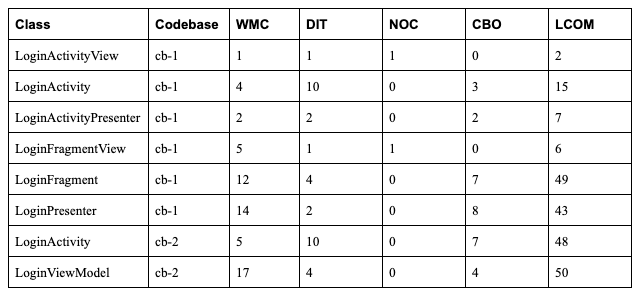
\includegraphics[scale=0.65]{figures/login-metric-table.png}
    \caption{CodeMR Metric Values for Login Feature}
    \label{fig:login-metric-table}
\end{figure}
\FloatBarrier

In order to examine the results better, groupings can be made between these classes, and the metric values of these groups can be compared. This grouping can be made based on the responsibilities of the classes. The responsibilities to be taken as a basis while groups are determined as view and view logic. More detailed information on these responsibilities was shared in previous sections. These classes and their interfaces can be grouped for each codebase as follows. For cb-1, LoginActivityView, LoginActivity, LoginFragmentView and LoginFragment are only responsible for the presentation of the data.  LoginActivityPresenter and LoginFragmentPresenter are the classes responsible for how and when the data is presented. For cb-2, LoginActivity is responsible for presenting data, and LoginViewModel is responsible for how and when data is presented. This grouping will be useful for comparing the metric values shared in Fig. \ref{fig:code-mr-metric-val}. In the table below, the metric values for each group of both codebases that are obtained from the analysis made within the scope of this study are shared.

\begin{figure}[ht!]
    \centering
    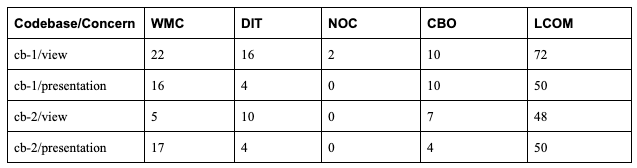
\includegraphics[scale=0.65]{figures/login-metric-table-2.png}
    \caption{CodeMR Metric Values for Login Feature}
    \label{fig:login-metric-table-2}
\end{figure}
\FloatBarrier